\chapter{Estudio técnico}

El desarrollo de este capítulo, que se basa en el estudio de mercado previo, es de vital importancia para determinar la viabilidad técnica de nuestro proyecto de empresa, que se dedicará a la construcción de cabinas climáticas para plantas. Este estudio se enfocará en su funcionamiento y operatividad, y entre sus principales objetivos se destacan los siguientes: 
\begin{itemize}
    \item Determinar la localización y tamaño óptimo de la infraestructura de la empresa. 
    \item Definir una distribución adecuada de las instalaciones de la maquinaria
    \item Determinar las especificaciones de los materiales e insumos, maquinaria y equipo para la definición de los procesos de producción de las cabinas, así como todos aquellos equipos necesarios para llevar a cabo el proceso administrativo. 
    \item Determinar los costos de las instalaciones, materiales e insumos, maquinaria, mano de obra y demás equipos, así como también, su oferta en el mercado.
    \item Determinar el proceso y programa de producción para el horizonte de vida del proyecto de las cabinas climáticas para plantas. 
\end{itemize}

El estudio técnico se presenta en dos secciones por cuestiones de metodología, en la primera, la localización y tamaño de la infraestructura de la empresa, y en la segunda, los aspectos referentes a la Ingeniería que conlleva.

\section{Localización óptima del proyecto}
La Localización Óptima del Proyecto es un componente esencial del estudio técnico que busca identificar el lugar más adecuado para establecer la infraestructura necesaria para la realización de las cabinas climáticas para plantas. Este análisis incluye:

\begin{itemize}
    \item Macrolocalización: Evaluación de la región o área geográfica amplia donde se situará la infraestructura del proyecto.
    \item Microlocalización: Análisis detallado del sitio específico dentro de la región seleccionada.
    \item Croquis de Localización: Una representación gráfica que ilustra la ubicación propuesta de la infraestructura.
\end{itemize}

\subsection{Macrolocalización}
La Macrolocalización de nuestra empresa de cabinas climáticas se centrará en la región de la Mixteca en el Estado de Oaxaca, una zona que, a pesar de su rica diversidad cultural y recursos naturales, enfrenta desafíos significativos como el desempleo y la migración. Según datos recientes, la tasa de desempleo en Oaxaca en el cuarto trimestre de 2023 fue del 1.54\% y la tasa de informalidad laboral alcanzó el 81.1\% \cite{DataMexico2023}. Estos indicadores resaltan la necesidad de proyectos innovadores que puedan generar empleo y estimular el desarrollo económico local.

Nuestro proyecto no solo busca ofrecer soluciones avanzadas para el cultivo de plantas, sino también crear oportunidades de trabajo y fomentar el crecimiento en la región. Con la implementación de la empresa en la Mixteca, aspiramos a contribuir positivamente al entorno socio-económico y reducir las tendencias de migración al proporcionar alternativas de empleo sustentables en la comunidad.

\begin{figure}[H]
    \centering	
    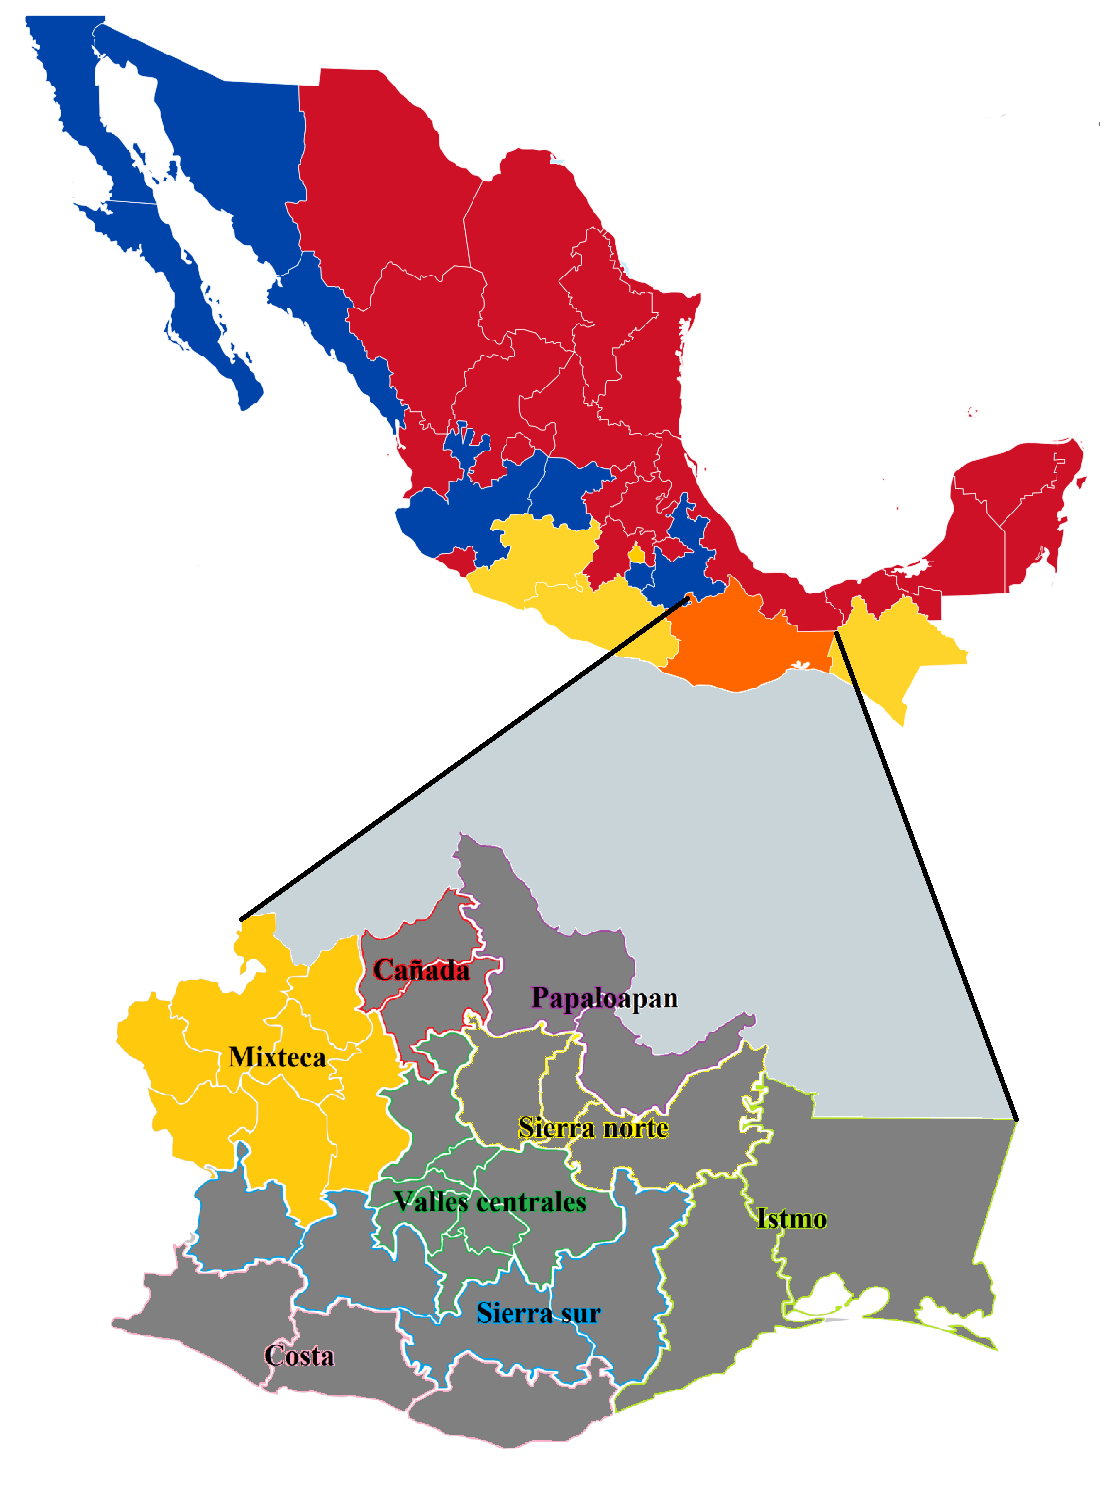
\includegraphics[width=.6\textwidth]{img/macrolocalizacion.png} 
    \caption{Plano de macro localización}
\label{fig:macrolocalizacion}
\end{figure}


\newpage


\subsection{Microlocalización}
Nuestra empresa de cabinas climáticas se enfocará en su sede en la Heroica Ciudad de Huajuapan de León, ubicada en la región Mixteca de Oaxaca. Esta ciudad es una opción estratégica por varias razones:

\textbf{Mercado:} Huajuapan de León cuenta con una población significativa y una actividad comercial vibrante, lo que la convierte en el principal mercado consumidor de la Mixteca.

\textbf{Materias Primas:} La ciudad es un punto de acceso clave para la Mixteca, conectada por las carreteras 190 y 125, facilitando la llegada de proveedores y materias primas desde la Ciudad de México y Puebla.

\begin{figure}[H]
    \centering	
    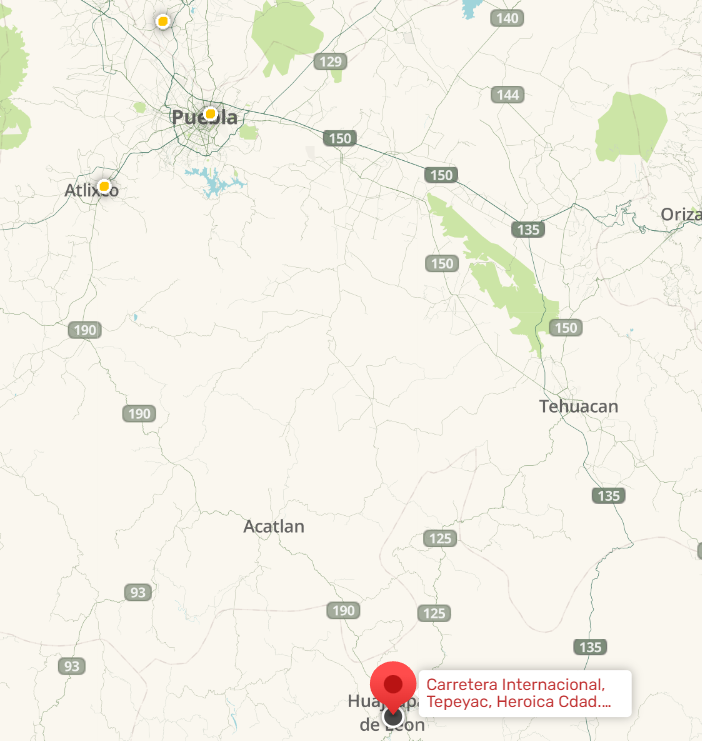
\includegraphics[width=.7\textwidth]{img/carretera190125.png} 
    \caption{Croquis Huajuapan}
\label{fig:croquis190125}
\end{figure}

\textbf{Mano de Obra:} A pesar de la migración, Huajuapan de León atrae a buscadores de empleo debido a su comercio activo, asegurando una oferta de mano de obra disponible para la producción de cabinas climáticas
\newpage

\begin{table}[h!]
\centering
\begin{tabular}{|l|l|}
\hline
\textbf{Infraestructura} & \textbf{Descripción} \\
\hline
Vías de Acceso & Carretera 190 y 125 (ver figura \ref{fig:croquis190125}) \\
\hline
Transporte Urbano & Servicios de autobuses y taxis \\
\hline
Abastecimiento de Agua & 78.3\% de las viviendas con acceso a agua entubada \\
\hline
Manejo de Residuos & Servicios de recolección de basura \\
\hline
Educación & Escuelas primarias, secundarias y universidades \\
\hline
Salud & Hospitales y clínicas locales \\
\hline
\end{tabular}
\caption{Infraestructura disponible en la ciudad de Huajuapan de León (Información Actualizada)}
\label{table:infrahuajuapan}
\end{table}

Como puede verse en la tabla \ref{table:infrahuajuapan}, la ciudad de Huajuapan de León cuenta con la infraestructura necesaria para la construcción de la empresa, destacando el acceso a internet de alta velocidad que recientemente se agregó en la ciudad, también cuenta con la Universidad Tecnológica de la Mixteca que ofrecería el acceso a un personal mejor capacitado. 

\subsection{Aspectos demográficos y económicos}
La región de Huajuapan de León, ubicada en el estado de Oaxaca, latitud: 17°48,28. N 
y longitud: 97°46,46. O, presenta características demográficas y económicas particulares que la hacen un lugar estratégico para el desarrollo de nuestro proyecto de cabinas climáticas para plantas.

Al norte colinda con el estado de Puebla y los municipios de Zapotitlán Palmas, Santiago Miltepec y Asunción Cuyotepeji, al este con los municipios de Asunción Cuyotepeji, Santa María Camotlán, Santiago Huajolotitlán y Santiago Cacaloxtepec, al sur con los municipios de Santiago Cacaloxtepec y San Marcos Arteaga, al oeste con los municipios San Marcos Arteaga, San Jerónimo Silacayoapilla, San Miguel Amatitlán, Santiago Ayuquililla, Zapotitlán Palmas y el estado de Puebla

En términos demográficos, Huajuapan de León ha experimentado un crecimiento poblacional significativo en los últimos años. Según el último censo, la población en 2020 fue de 78,313 habitantes, lo que representa un crecimiento del 12.1\% \cite{PoblacionHuajuapan2020} en comparación con 2010. de la población total, el 47.5\% son hombres y el 52.5\% son mujeres

En cuanto a la economía, la Inversión Extranjera Directa (IED) en Oaxaca alcanzó los US\$43.9M en el periodo de enero a diciembre de 2023, lo que indica un ambiente favorable para el desarrollo de proyectos empresariales.

Además, la tasa de desempleo en Oaxaca en el cuarto trimestre de 2023 fue del 1.54\%, lo que sugiere la disponibilidad de mano de obra en la región. Sin embargo, es importante destacar que la tasa de informalidad laboral alcanzó el 81.1\% \cite{DataMexicoHuajuapan2023}, lo que representa un desafío en términos de equidad laboral.

Estos aspectos demográficos y económicos son fundamentales para entender el entorno en el que se desarrollará nuestro proyecto y para diseñar estrategias que permitan maximizar su impacto en la región.

\subsection{Croquis de localización}
Nuestra área de interés dentro de la ciudad de Huajuapan de León es en un lugar cerca del centro pero a su vez que esté en las orillas, es por eso que se decidió usar las antiguas instalaciones del grupo PEPSICO, ya que está a un costado de la carretera 190 y además ya cuenta con la mayoría de la infraestructura realizada, por lo que solamente se reacondicionaría el lugar y construir las áreas faltantes. 

Se ubica en la colonia el Tepeyac, Juan Diego \#19, esquina con Díaz Ordaz.

\begin{figure}[H]
    \centering	
    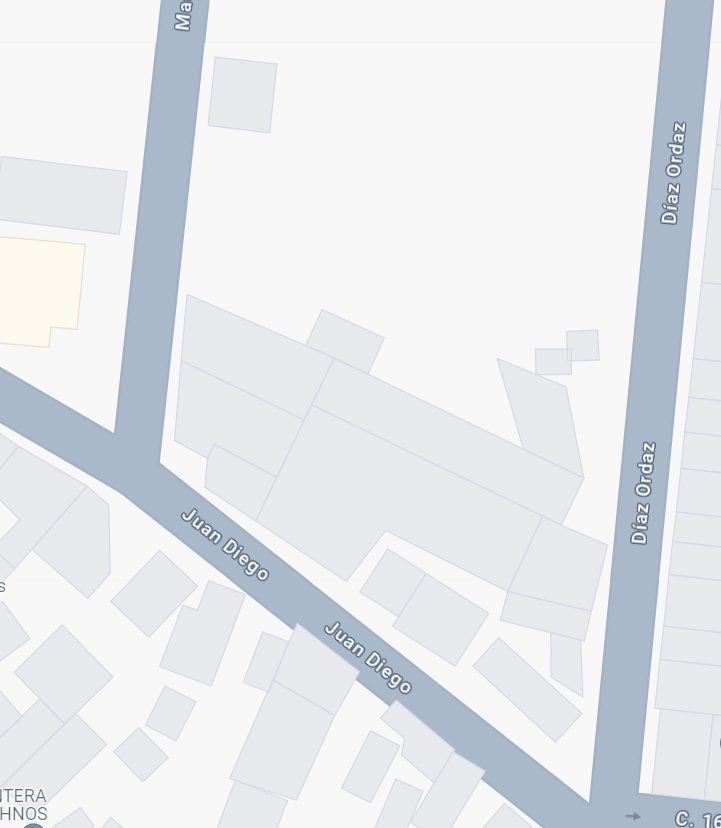
\includegraphics[width=.7\textwidth]{img/Empresa/ubicacion1.png} 
    \caption{Croquis de la localización de la empresa}
\label{fig:croquis1}
\end{figure}

\begin{figure}[H]
    \centering	
    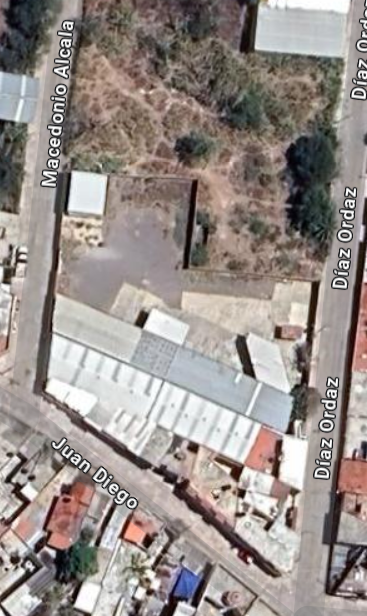
\includegraphics[width=.7\textwidth]{img/Empresa/ubicacion2.png} 
    \caption{Croquis satelital de la localización de la empresa}
\label{fig:croquis1}
\end{figure}

\newpage

\section{Capacidad óptima de producción}

La capacidad de producción es el volumen máximo de productos que puede generar una planta o empresa de manufactura en un período determinado, utilizando los recursos disponibles. Es crucial para calcular el rendimiento financiero futuro y establecer una línea de tiempo confiable para la entrega de los productos.

   \begin{itemize}
       \item Se llevó a cabo un estudio exhaustivo del mercado de cabinas para el cuidado de plantas, incluyendo la revisión de informes de la industria, análisis de tendencias de consumo y entrevistas con expertos del sector.
       \item Se recopiló información sobre la demanda actual y proyectada de cabinas para el cuidado de plantas, considerando factores demográficos, hábitos de consumo y tendencias de estilo de vida.
       \item Se identificaron segmentos de mercado clave, como propietarios de viviendas, entusiastas de la jardinería, restaurantes y hoteles, para comprender sus necesidades y preferencias.
   \end{itemize}

\subsection{Capacidad de producción actual}


La empresa \textbf{“Terra Green”} se especializa en la fabricación de cabinas diseñadas para el cuidado óptimo de plantas en entornos controlados. Según los datos recabados en la proyección de la demanda (página 8), se estima una demanda de \textbf{280,000 unidades en el primer año}. Sin embargo, Terra Green ha decidido satisfacer solo el \textbf{5 por ciento de esa demanda}, lo que implica producir \textbf{14,000 unidades al año} o \textbf{1,167 unidades al mes}.

Para diseñar un sistema de producción con un máximo de \textbf{3 por ciento de error}, se espera una producción de \textbf{1,203 unidades al mes}, lo que se traduce en \textbf{300 unidades por semana} o \textbf{60 unidades al día}.

\textbf{Parámetros de Producción:}
\begin{itemize}
    \item \textbf{Jornada Laboral:} Se propone una jornada de 16 horas (dos turnos) sin cargo extra según CFE.
    \item \textbf{Capacidad de Producción por Hora:} Se espera que cada hora se produzcan 3.75 unidades.
    \item \textbf{Tiempo de Producción por Pieza:} El tiempo de producción total por cada pieza es de 16 minutos, siendo esta la máxima capacidad de producción.
\end{itemize}

\textbf{Diseño y Características de las Cabinas:}
\begin{itemize}
    \item \textbf{Espacio Interior:} Las cabinas se diseñarán en diferentes tamaños para acomodar una variedad de plantas, desde pequeñas hierbas hasta árboles frutales en macetas. Se utilizarán materiales transparentes (vidrio o plástico) para permitir la entrada de luz natural y la observación de las plantas.
    \item \textbf{Sistemas de Control Ambiental:} Se incorporarán sensores de temperatura, humedad y luz para monitorear y ajustar automáticamente las condiciones internas. Los sistemas de riego automático y ventilación serán parte integral del diseño.
    \item \textbf{Materiales y Construcción:} Las cabinas se construirán con paneles aislantes para mantener una temperatura constante. Se utilizarán materiales reciclables y sostenibles siempre que sea posible.
    \item \textbf{Eficiencia Energética:} Se implementarán luces LED de bajo consumo energético para la iluminación interna. El sistema de calefacción y refrigeración se optimizará para minimizar el gasto energético.
\end{itemize}

\textbf{Beneficios para los Clientes:}
\begin{itemize}
    \item Las cabinas de Terra Green ofrecerán un entorno ideal para el crecimiento de plantas en interiores.
    \item Los usuarios podrán cultivar hierbas, flores y vegetales durante todo el año, independientemente del clima exterior.
    \item La durabilidad y eficiencia energética garantizarán una inversión a largo plazo.
\end{itemize}




  

\section{Ingeniería del proyecto}

\subsection{Proceso de Producción}

\begin{itemize}
    \item \textbf{Diseño y Planificación:}
    \begin{itemize}
        \item El equipo de diseño de Terra Green crea los planos y especificaciones detalladas para las cabinas. Esto incluye el tamaño, la disposición interna, los materiales y los sistemas de control ambiental.
        \item Se definen los parámetros clave, como la capacidad de producción, el tiempo de producción por pieza y la jornada laboral.
    \end{itemize}
    
    \item \textbf{Adquisición de Materiales:}
    \begin{itemize}
        \item Se adquieren los materiales necesarios para la construcción de las cabinas. Esto puede incluir paneles de vidrio o plástico transparente, aislantes, sensores, luces LED y otros componentes.
    \end{itemize}
    
    \item \textbf{Fabricación de Componentes:}
    \begin{itemize}
        \item Se fabrican los componentes básicos de las cabinas, como los paneles laterales, las puertas, los estantes y los sistemas de iluminación.
        \item Los sistemas de control ambiental (sensores, sistemas de riego, ventilación) también se ensamblan y prueban.
    \end{itemize}
    
    \item \textbf{Ensamblaje de las Cabinas:}
    \begin{itemize}
        \item Se ensamblan las cabinas siguiendo los planos de diseño. Se unen los paneles, se instalan las puertas y se conectan los sistemas de control.
        \item Se aplican los acabados exteriores y se asegura la estabilidad y durabilidad de cada cabina.
    \end{itemize}
    
    \item \textbf{Control de Calidad:}
    \begin{itemize}
        \item Cada cabina pasa por un riguroso control de calidad. Se verifica que todos los componentes funcionen correctamente y que las condiciones internas sean las adecuadas.
        \item Se realizan pruebas de resistencia, eficiencia energética y seguridad.
    \end{itemize}
    
    \item \textbf{Embalaje y Almacenamiento:}
    \begin{itemize}
        \item Las cabinas se embalan cuidadosamente para su transporte. Se protegen contra daños durante el envío.
        \item Se almacenan en el área de distribución hasta su entrega a los clientes.
    \end{itemize}
    
    \item \textbf{Entrega y Montaje:}
    \begin{itemize}
        \item Las cabinas se entregan a los clientes según sus pedidos. El equipo de instalación de Terra Green se encarga del montaje en el lugar deseado.
        \item Se realizan pruebas finales para asegurar que todo funcione correctamente.
    \end{itemize}
    
    \item \textbf{Servicio Postventa:}
    \begin{itemize}
        \item Terra Green ofrece soporte técnico y mantenimiento a sus clientes. Cualquier problema o ajuste necesario se atiende de manera rápida y eficiente.
    \end{itemize}
\end{itemize}

\subsection{Distribución de planta}

El proyecto de la empresa constructora de cabinas para el cuidado de plantas en México es de gran envergadura, considerando la creciente demanda de soluciones de jardinería urbana y el interés cada vez mayor en el cultivo de plantas en interiores.

Para satisfacer esta demanda, la empresa planea establecer una planta de producción de tamaño considerable en una ubicación estratégica, que permita el acceso fácil a materias primas y mano de obra calificada, así como una logística eficiente para la distribución de los productos terminados.

Además, se contempla la posibilidad de ampliar las instalaciones en el futuro para aumentar la capacidad de producción y diversificar la oferta de productos, incluyendo diferentes tamaños y diseños de cabinas para satisfacer las necesidades de diversos segmentos de mercado.


La distribución de la planta de producción se ha diseñado cuidadosamente para optimizar el flujo de materiales y minimizar los tiempos muertos en el proceso de fabricación.

En primer lugar, se han establecido áreas dedicadas para cada etapa del proceso de producción, desde el almacenamiento de materias primas hasta el ensamblaje final y las pruebas de calidad. Esto permite una organización eficiente del trabajo y facilita la supervisión y el control de cada fase del proceso.

Además, se han implementado sistemas de transporte interno, como cintas transportadoras y carretillas elevadoras, para facilitar el movimiento de materiales entre las diferentes áreas de la planta. Esto reduce el tiempo de manipulación de materiales y aumenta la productividad general de la planta.

Por último, se han instalado equipos de seguridad y medidas de prevención de accidentes en toda la planta para garantizar un entorno de trabajo seguro y cumplir con las regulaciones laborales vigentes en México



\begin{table}[H]
    \centering
    \caption{Actividades, Descripción y Equipo Necesario para la Producción de Cabinas}
    \begin{tabular}{|l|p{0.4\textwidth}|p{0.4\textwidth}|}
        \hline
        \textbf{Actividad} & \textbf{Descripción de la Actividad} & \textbf{Equipo Necesario} \\
        \hline
        Diseño y Planificación & Creación de planos y especificaciones detalladas para la cabina. Incluye tamaño, disposición interna y sistemas de control ambiental. & Equipo de diseño, software de diseño asistido por computadora (CAD). \\
        \hline
        Adquisición de Materiales & Compra de materiales necesarios para la construcción de la cabina. Incluye paneles de vidrio o plástico transparente, aislantes, sensores, luces LED, etc. & Departamento de compras, proveedores. \\
        \hline
        Fabricación de Componentes & Producción de partes básicas de la cabina, como paneles laterales, puertas, estantes y sistemas de iluminación. & Máquinas de corte, soldadoras, herramientas manuales. \\
        \hline
        Ensamblaje de las Cabinas & Montaje de la cabina siguiendo los planos de diseño. Unión de paneles, instalación de puertas y conexión de sistemas de control. & Herramientas de ensamblaje, personal de producción. \\
        \hline
        Control de Calidad & Verificación de que todos los componentes funcionen correctamente y que las condiciones internas sean adecuadas. Pruebas de resistencia, eficiencia energética y seguridad. & Personal de calidad, equipos de prueba. \\
        \hline
        Embalaje y Almacenamiento & Empaque cuidadoso de la cabina para transporte. Protección contra daños durante el envío. Almacenamiento en área de distribución. & Materiales de embalaje, área de almacenamiento. \\
        \hline
        Entrega y Montaje & Entrega de la cabina al cliente según pedido. Montaje en el lugar deseado por el equipo de instalación. & Personal de entrega, herramientas de montaje. \\
        \hline
        Servicio Postventa & Soporte técnico y mantenimiento para los clientes. Atención rápida y eficiente a problemas o ajustes. & Personal de servicio al cliente, herramientas de reparación. \\
        \hline
    \end{tabular}
\end{table}


\section*{Planta Arquitectónica del Proyecto}

\subsection*{\textbf{Descripción por Área}}

\begin{itemize}
    \item \textbf{Recepción de Materiales:}
    \begin{itemize}
        \item \textbf{Dimensión:} 150 m\textsuperscript{2}
        \item \textbf{Ubicación:} En la entrada principal de la planta.
        \item \textbf{Conexiones:} Con el área de corte de materiales y el área de almacenamiento.
    \end{itemize}

    \item \textbf{Corte de Materiales:}
    \begin{itemize}
        \item \textbf{Dimensión:} 960 m\textsuperscript{2}
        \item \textbf{Ubicación:} Adyacente a la recepción de materiales.
        \item \textbf{Conexiones:} Con el área de montaje de estructuras y el área de instalación de sistemas.
    \end{itemize}

    \item \textbf{Montaje de Estructura:}
    \begin{itemize}
        \item \textbf{Dimensión:} 2000 m\textsuperscript{2}
        \item \textbf{Ubicación:} Contigua al área de corte de materiales.
        \item \textbf{Conexiones:} Con el área de pruebas de calidad y el área de empacado y almacenamiento.
    \end{itemize}

    \item \textbf{Instalación de Sistemas:}
    \begin{itemize}
        \item \textbf{Dimensión:} 1280 m\textsuperscript{2}
        \item \textbf{Ubicación:} Junto al área de corte de materiales.
        \item \textbf{Conexiones:} Con el área de montaje de estructuras y el área de pruebas de calidad.
    \end{itemize}

    \item \textbf{Pruebas de Calidad:}
    \begin{itemize}
        \item \textbf{Dimensión:} 400 m\textsuperscript{2}
        \item \textbf{Ubicación:} Al lado del área de montaje de estructuras.
        \item \textbf{Conexiones:} Con el área de instalación de sistemas y el área de empacado y almacenamiento.
    \end{itemize}

    \item \textbf{Empaque y Almacenamiento:}
    \begin{itemize}
        \item \textbf{Dimensión:} 400 m\textsuperscript{2}
        \item \textbf{Ubicación:} Adyacente al área de pruebas de calidad.
        \item \textbf{Conexiones:} Con el área de montaje de estructuras y el área de corte de materiales.
    \end{itemize}

    \item \textbf{Estacionamiento para Empleados:}
    \begin{itemize}
        \item \textbf{Dimensión:} 500 m\textsuperscript{2}
        \item \textbf{Ubicación:} Junto a la entrada principal de la planta.
    \end{itemize}

    \item \textbf{Oficinas Administrativas:}
    \begin{itemize}
        \item \textbf{Dimensión:} 600 m\textsuperscript{2}
        \item \textbf{Ubicación:} En un área central de la planta.
    \end{itemize}

    \item \textbf{Área de Descanso:}
    \begin{itemize}
        \item \textbf{Dimensión:} 200 m\textsuperscript{2}
        \item \textbf{Ubicación:} Cerca de las oficinas administrativas.
    \end{itemize}
\end{itemize}

\subsection*{\textbf{Dimensión Total de la Planta:} 6690 m\textsuperscript{2}}




\newpage

\section{Inversión fija}




\begin{figure}[H]
    \centering	
    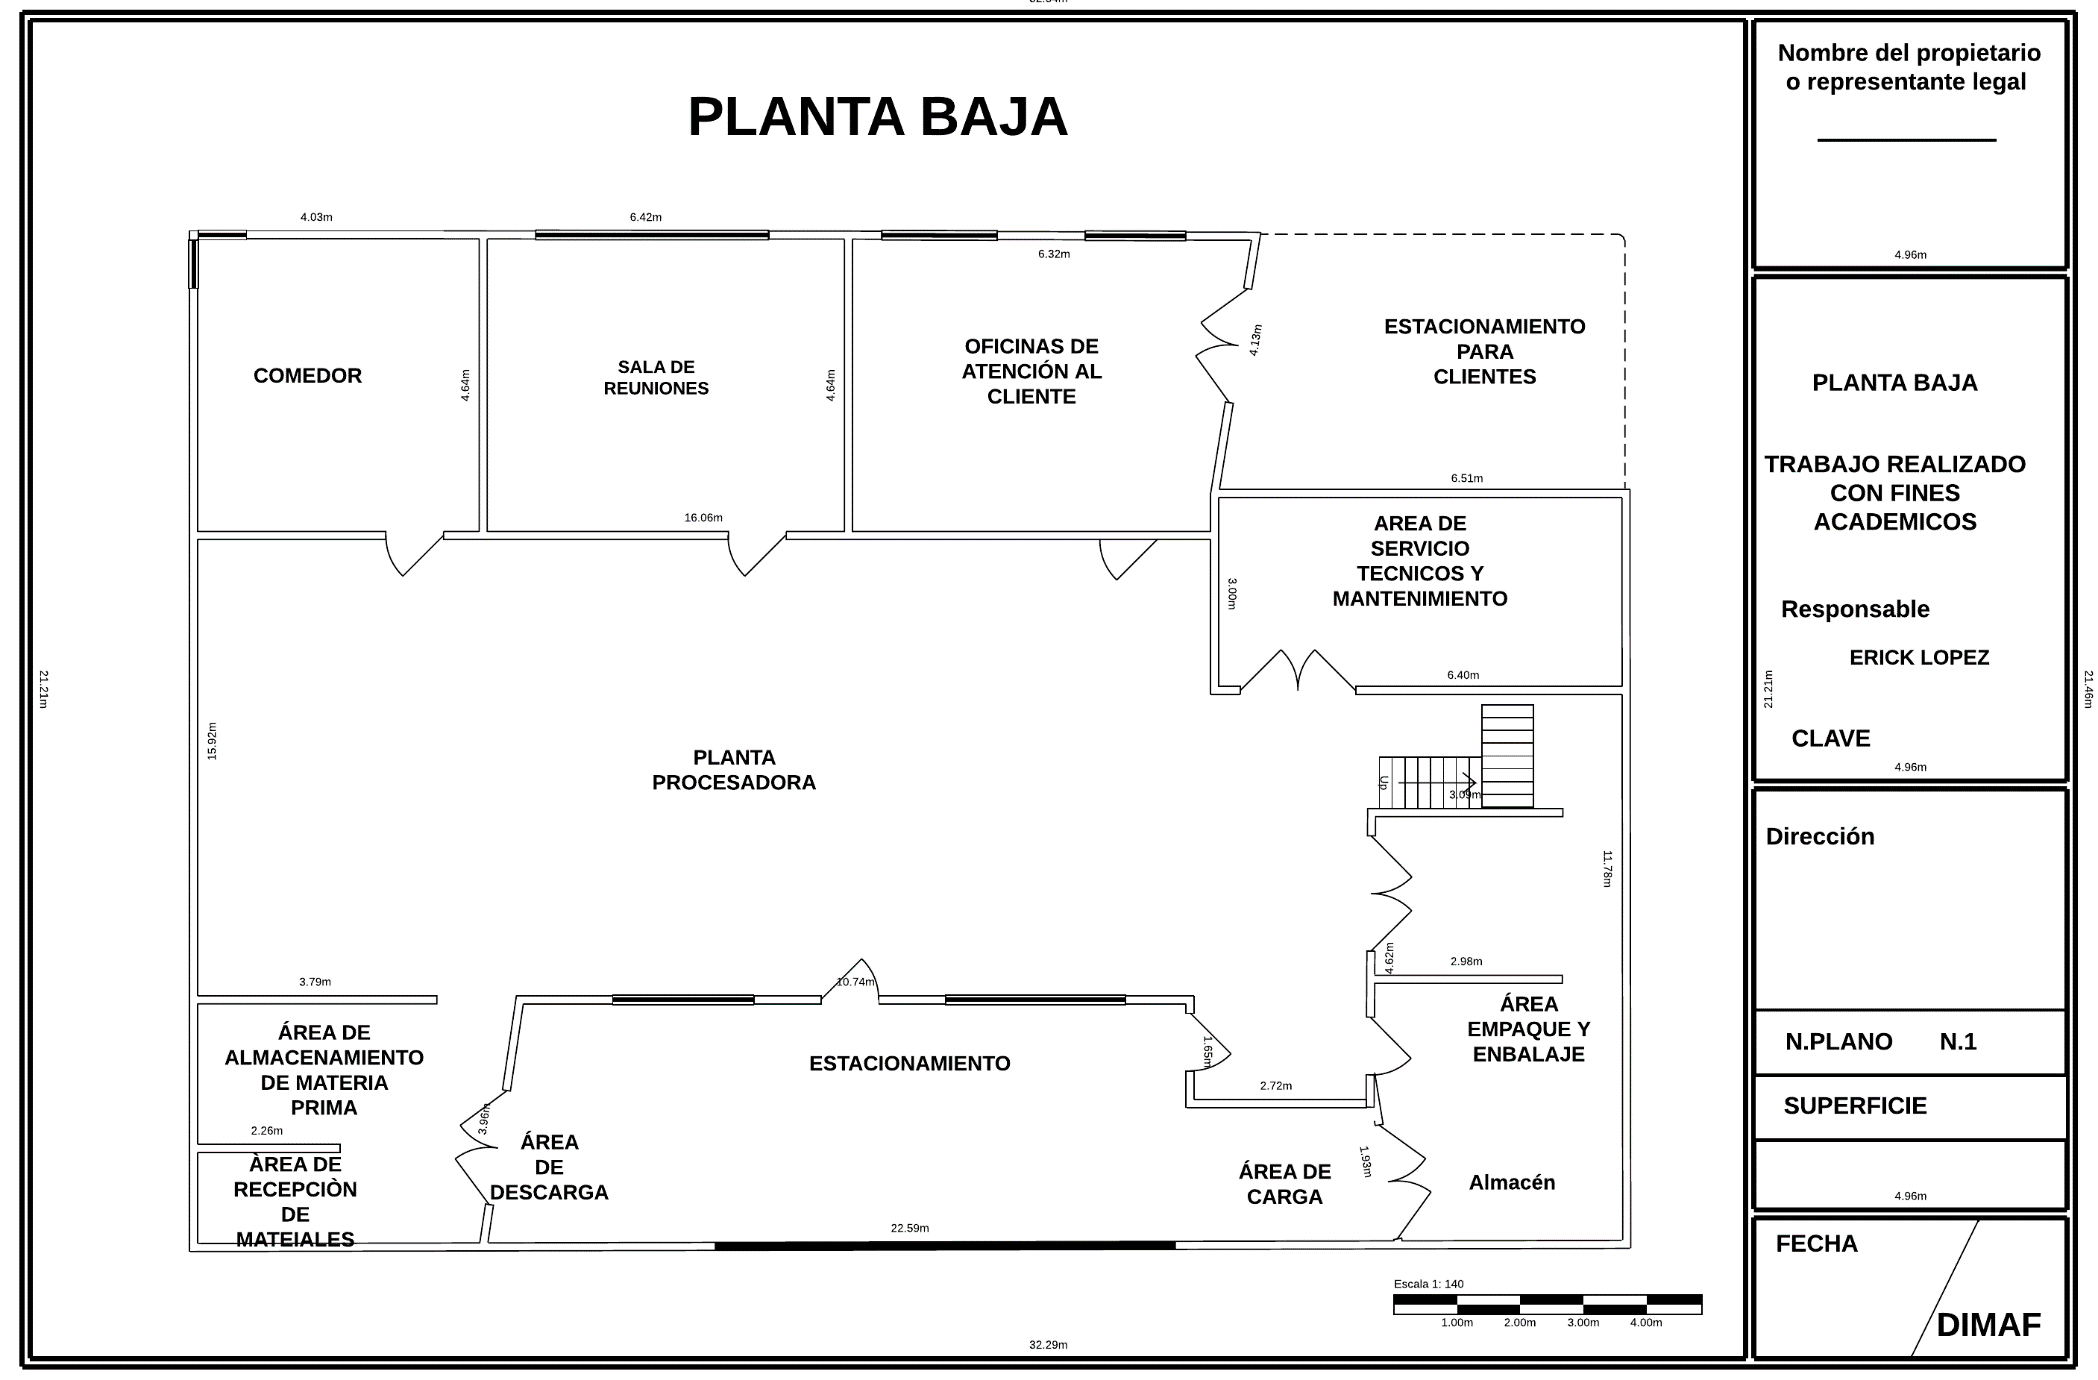
\includegraphics[angle=90,width=1.0\textwidth]{chapters/image1_.png} 
    \caption{Planta baja}
\label{fig:croquis190125}
\end{figure}

\begin{figure}[H]
    \centering	
    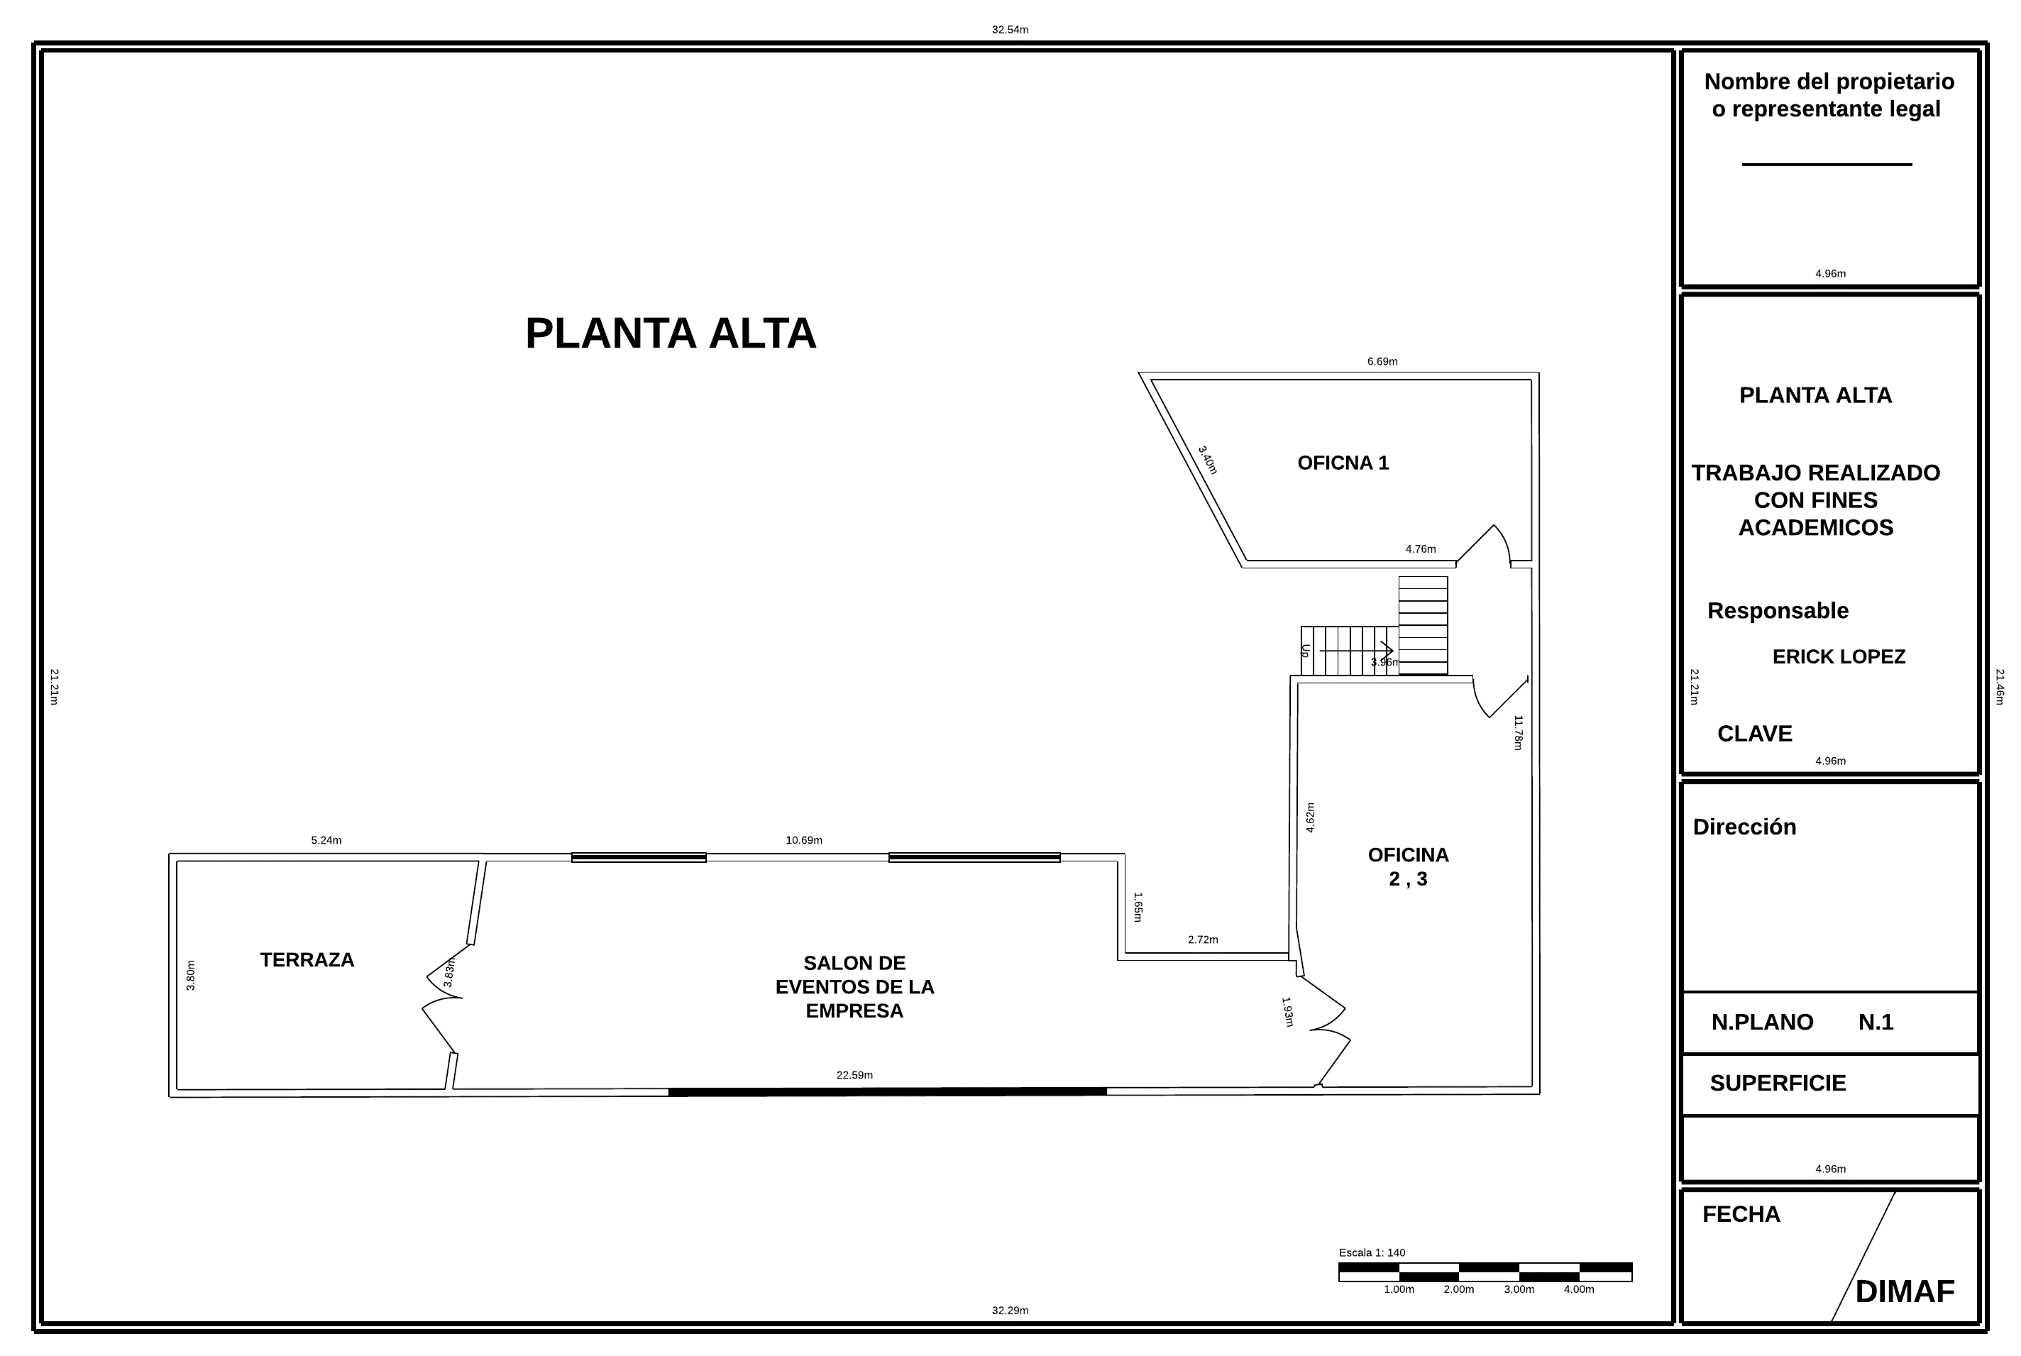
\includegraphics[angle=90,width=1.0\textwidth]{chapters/image2_.png} 
    \caption{Planta alta}
\label{fig:croquis190125}
\end{figure}

\begin{figure}[H]
    \centering	
    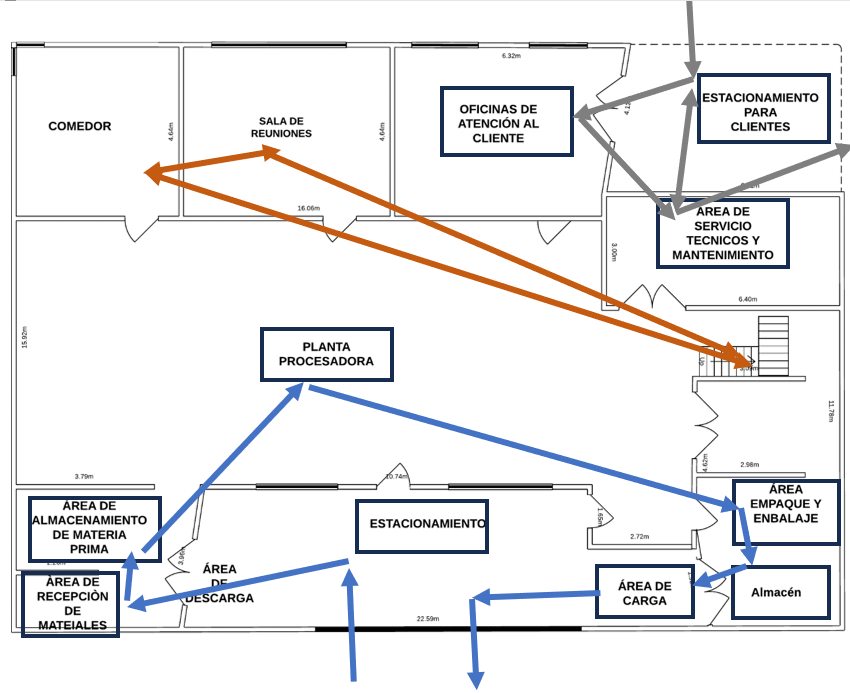
\includegraphics[angle=90,width=0.75\textwidth]{chapters/ELC_HILOS.png} 
    \caption{Diagrama de hilos}
\label{fig:croquis190125}
\end{figure}

Se tienen 3 principales hilos los cuales comprenden a 

1. Color gris

Es cuando una persona externa visita la empresa y esta desea un servicio técnico, atención a cliente o un acercamiento más a la empresa.

2. Color naranja

Área que recorre el personal administrativo y estos se conectan directamente a la segunda planta con las demás áreas administrativas.

3. Color azul 

Es la ruta que toman la contracción del producto desde recepción de materia prima hasta la entrega el producto final este camino es unidireccional, ya que no se puede regresar el material a un estado anterior. 

\begin{figure}[H]
    \centering	
    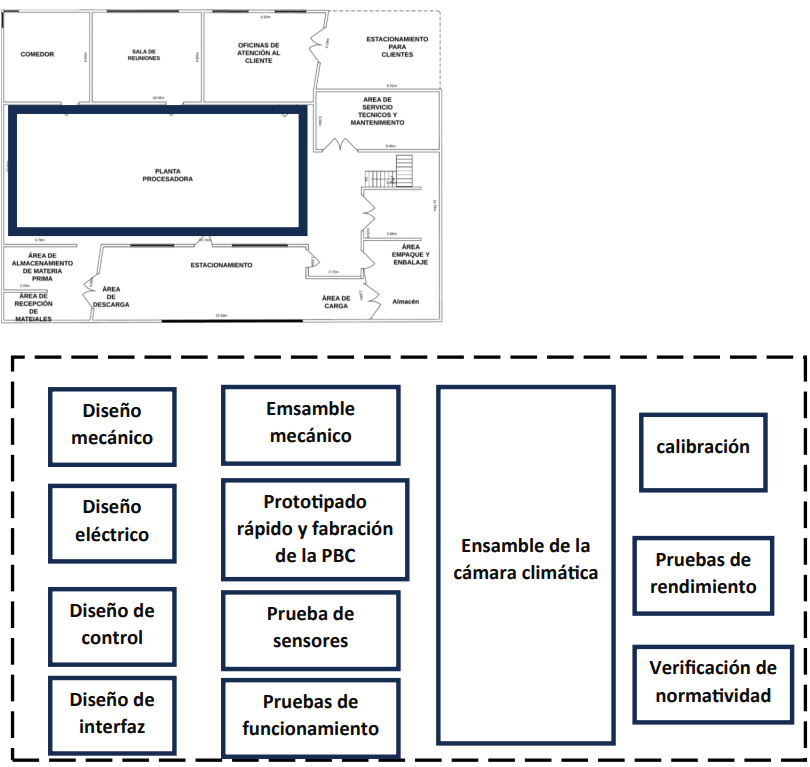
\includegraphics[angle=0,width=0.67\textwidth]{chapters/ELC_DIAGRAM.png} 
    \caption{Diagrama de distribución del área de producción}
\label{fig:croquis190125}
\end{figure}

Para poder producir las cámaras climáticas en necesario tener una distribución uniforme y las áreas no deben de estar alejadas, ya que nos reduce el tiempo de movimiento de materiales además de poder interactuar con las demás área para un correcto flujo y detección de errores.

\begin{figure}[H]
    \centering	
    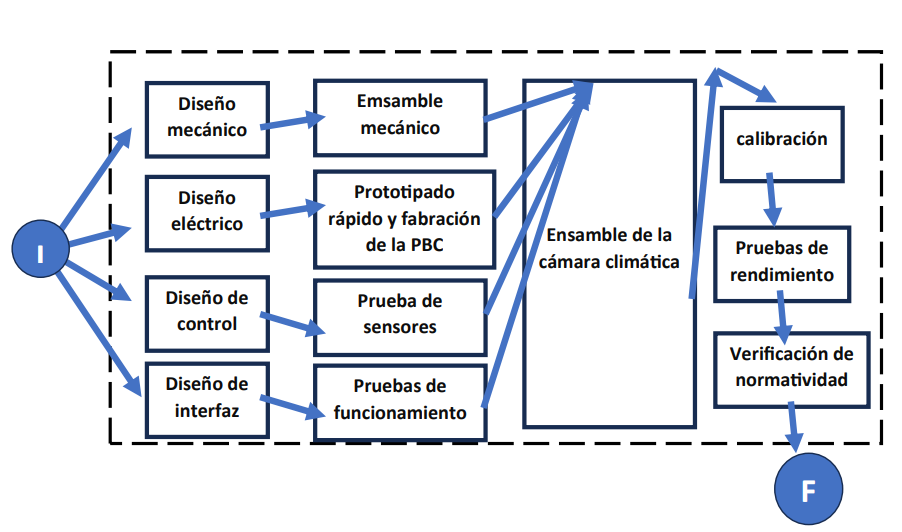
\includegraphics[angle=0,width=0.70\textwidth]{chapters/ELC_DIAGRAM2.png} 
    \caption{Diagrama hilos de la distribución del área de producción}
\label{fig:croquis190125}
\end{figure}

Se diseñó el área de producción para poder tener 4 áreas en este caso trabajando al mismo tiempo para aumentar efectividad y reducir los tiempos con ello podemos desarrollar productos más rápidos y permitir realizar productos personalizados cuando sea su caso. 
%----------------------------------------





\subsection{Adquisición del equipo de transporte}

Este punto implica la compra de equipos de transporte como transportadores de banda, carretillas elevadoras, o cualquier otro equipo necesario para el movimiento de materias primas, productos semiacabados y productos terminados dentro de la planta.

Se debe considerar la capacidad de carga, la eficiencia energética y la seguridad de estos equipos al seleccionarlos.

La inversión en equipos de transporte adecuados es crucial para garantizar un flujo de trabajo eficiente y minimizar los tiempos de inactividad en la planta.

\begin{table}[htbp]
    \centering
    \begin{tabular}{|l|c|c|c|}
        \hline
        \textbf{Concepto}               & \textbf{Cantidad} & \textbf{Costo Unitario} & \textbf{Importe} \\
        \hline
        Transportador de banda          & 2                 & \$10,000.00              & \$20,000.00      \\
        Carretilla elevadora eléctrica & 1                 & \$15,000.00              & \$15,000.00      \\
        Plataforma móvil                & 1                 & \$8,000.00               & \$8,000.00       \\
        \hline
        Subtotal                        &                   &                          & \$43,000.00      \\

        IVA (16\%)                      &                   &                          & \$6,880.00       \\
        \hline
        TOTAL                           &                   &                          & \$49,880.00      \\
        \hline
    \end{tabular}
    \caption{Adquisición de Equipo de Transporte}
    \label{tab:equipo_transporte}
\end{table}

Se considera la adquisición de una plataforma móvil que puede ser útil para tareas de mantenimiento o para acceder a áreas elevadas dentro de la planta.

El subtotal muestra el costo total de todos los elementos de equipo de transporte, mientras que el IVA representa el impuesto sobre el valor agregado aplicable. El total general refleja el costo total, incluido el impuesto.

\subsection{Adquisición de herramientas y refacciones}

Este punto implica la compra de herramientas específicas necesarias para el mantenimiento y la reparación de equipos, así como para llevar a cabo tareas operativas diarias.
Además de las herramientas, la adquisición de refacciones es esencial para garantizar la disponibilidad de piezas de repuesto para equipos críticos y minimizar el tiempo de inactividad en caso de averías.

\begin{table}[htbp]
    \centering
    \begin{tabular}{|l|c|c|c|}
        \hline
        \textbf{Concepto}               & \textbf{Cantidad} & \textbf{Costo Unitario} & \textbf{Importe} \\
        \hline
        Juego de llaves métricas       & 3 juegos          & \$200.00                 & \$600.00         \\
        Juego de destornilladores      & 3 juegos          & \$150.00                 & \$450.00         \\
        Equipo de soldadura            & 1                 & \$1,000.00               & \$1,000.00       \\
        Equipo de medición             & 1                 & \$800.00                 & \$800.00         \\
        Piezas de repuesto    & Varios            & \$500.00                 & \$2,000.00       \\
        \hline
        Subtotal                       &                   &                          & \$4,850.00       \\
        IVA (16\%)                     &                   &                          & \$776.00         \\
        \hline
        TOTAL                          &                   &                          & \$5,626.00       \\
        \hline
    \end{tabular}
    \caption{Adquisición de Herramientas y Refacciones}
    \label{tab:herramientas_refacciones}
\end{table}

El equipo de soldadura es necesario para realizar reparaciones en caso de daños en componentes metálicos, mientras que el equipo de medición es esencial para garantizar la precisión en la instalación y ajuste de equipos.

Tambien se considera la compra de piezas de repuesto, lo que garantiza la disponibilidad de repuestos en caso de averías o fallos en los componentes críticos para el sistema de control de planta.




\section{Sistema de producción}
\subsection{Requerimientos técnicos del producto}

Entre los principales requerimientos del producto están:

\begin{itemize}
    \item Dimensiones de 0.5mx0.5mx0.8m
    \item Respetar la norma NOM 059 SEMARNAT-2010.
    \item El contenedor se construirá con material que brinde seguridad tanto a la planta como al usuario.
\end{itemize}

\subsubsection{Materias primas primarias.}

En la anterior sección \textbf{Análisis de la materia prima (pg. 3)} se nombran algunos materiales esenciales en la elaboración del producto, sin embargo aquí se enlistan las primarias.

\begin{itemize}
    \item Madera
    \item Acrílico
    \item Tornillos
    \item Adhesivo
\end{itemize}

\subsubsection{Materiales indirectos}

\begin{itemize}
    \item \textbf{Envases primarios:} Se planea entregar el producto final ensamblado aunque esto signifique una mayor demanda de transporte. El transporte llevará el producto final empaquetado en una caja de madera rellena de un material que evite daños al momento de ser transportada.
    \item \textbf{Envases secundarios:} Al momento del transporte, se pueden estibar un máximo de unidades y se pude hacer uso de tiras de plástico para hacer la estructura más estable.
\end{itemize}



\begin{figure}[H]
    \centering	
    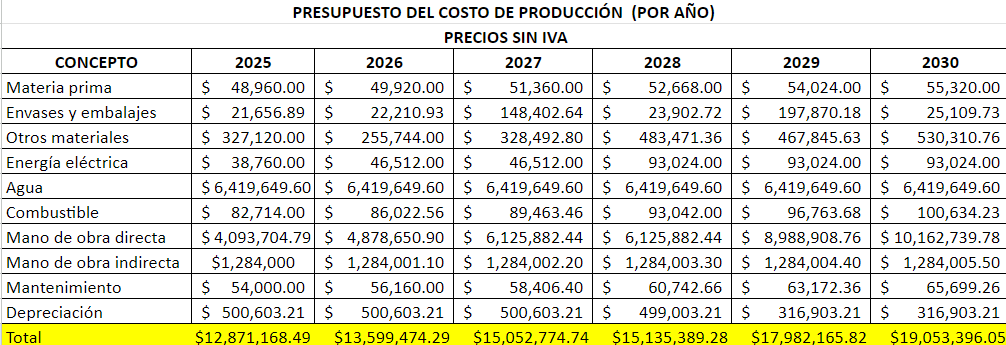
\includegraphics[angle=0,width=0.9\textwidth]{chapters/ELC_Produccion.png} 
    \caption{Costo de producción por año}
\label{fig:croquis190125}
\end{figure}



\subsection{Costo unitario}

Como se estimó en la sección \textbf{Análisis de precio (pg. 12)}, se toman en cuenta los datos de varios modelos disponibes en plataformas de comercio internacional y se cuenta con un precio aproximado de \$6,000, sin embargo, el producto ofrece más funciones con los que no cuenta la competencia, así que se puede establecer un precio de aproximadamente \$8,000, teniendo un margen de ganancia de \$2,500 por producto

\begin{figure}[H]
    \centering	
    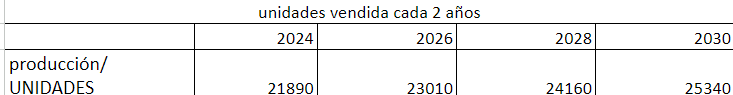
\includegraphics[angle=0,width=0.9\textwidth]{chapters/ELC_Unidades+.png} 
    \caption{Unidades de producción cada dos años}
\label{fig:croquis190125}
\end{figure}

\newpage



\newpage

\section{Conclusiones del estudio técnico}

Con el estudio técnico se encontró la tecnología adecuada para aplicar al desarrollo de las cámaras climáticas así como la evaluación de la disponibilidad de componentes en el mercado par asegurar una cadena de suministro estable, se evaluó el costo de producción por año como el de una unidad para poder comparar los pecios contra el mercado. Para poder operar de manera fácil y poder acceder a los usuarios finales se realizó la evaluación para la ubicación de la empresa. Ahora para poder tener el espacio suficiente y una adecuada distribución se optó por el desarrollo de la planta. Para poder iniciar a producir se requerirá tecnología de producción a lo cual se analizó el costo de la maquinaria así como de las diferentes áreas técnicas y administrativas.